%!TEX root = maindocument.tex

\block{Comparison of predicted and GFN2--xTB Hessian}{
	\Large
	\vspace{-2cm}
	\begin{minipage}{0.6\linewidth}
		\begin{itemize}
			\item Example: Hessian matrix of methane
			\item Overall good resemblance of the predicted Hessian compared to the computed GFN2--xTB Hessian.
		\end{itemize}	
	\end{minipage}%
	\begin{minipage}{0.4\linewidth}
		\vspace{2cm}
		\hspace*{3cm}
		\adjincludegraphics[height=10cm,trim={{.2\width} {.3\height} {.3\width} {.35\height}},clip]{Graphics/methane.eps}
	\end{minipage}
	\vspace*{-2cm}
	\begin{tikzfigure}
		\hspace{-2cm}
		\begin{minipage}{0.3\linewidth}
			\begin{flushleft}
				\hspace*{1.4cm}
				Model~
\includegraphics[width=30pt]{Graphics/blauerBlock.pdf}\\
			\end{flushleft}
		\begin{flushright}
			RMSD = 0.045 a.u.\\
		\end{flushright}

		\begin{flushleft}
				\hspace*{1.4cm}
				Model~
\includegraphics[width=30pt]{Graphics/roterBlock.pdf}\\
			\end{flushleft}
		\begin{flushright}
			RMSD = 0.015 a.u.\\
		\end{flushright}
		\end{minipage}%
		\hspace*{0.5cm}
		\begin{minipage}{0.7\linewidth}
			\vspace{0.7cm}
			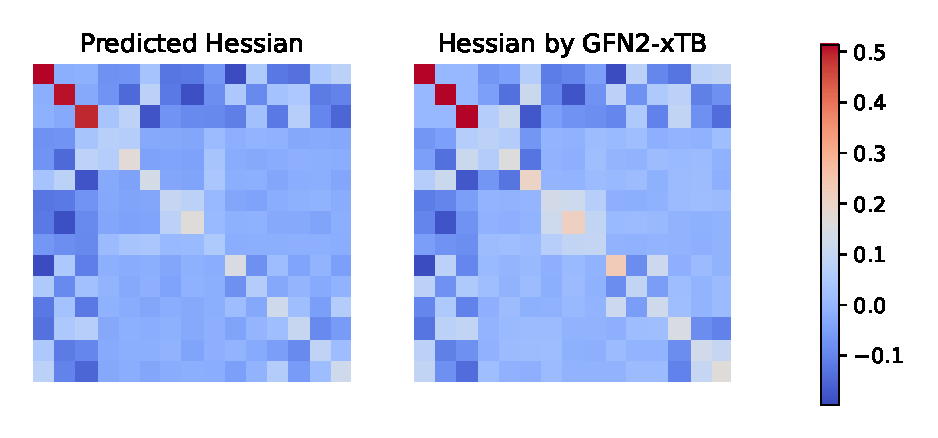
\includegraphics[width=\linewidth]{Graphics/ComparisonHessian.eps}
		\end{minipage}
	\end{tikzfigure}
	   }
	   
	   
	   
	   